\documentclass[../main.tex]{subfiles}
 
\begin{document}
\textbf{Indels in \textit{Armillaria gallica}}

Through previous studies on the \textit{Armillaria gallica} fungus, several strains were sequenced in Illuminia. These strains were analyzed using samtools and an additional package called bcftools. 

Through the use of bcftools, labels were added to the output which indicated various other information about the indel found such as: maximum number of reads supporting an indel, raw read depth, the number of reads that support the indel and other information.

As seen in \ref{tab:sum_indel}, many indels are found throughout most if not all of the strains analyzed. The summary table only shows the first three indels found within the each strain, however throughout the data, this is a repeated pattern. Indels are shown to be shared amongst the strains. 

\begin{table}[H]
\begin{center}
	\vspace{-1.5cm}
	\begin{singlespace}
		\captionof{table}[Summary Indel Table]{A summary table of the first three indels found in each of the strains which includes the scaffold number, the location at which the indel is found, the number of reads that support that indel, and the raw read depth\\} \label{tab:sum_indel}
	\scalebox{.9}{
	\begin{tabular}{ |c|c|c|c|c|c|c| } 
		\hline
		Strain No. & Scaffold No. & Location & No. of Reads Supporting & Raw Read Depth \\
		\hline
		\multirow{3}{4em}{Ar73} & 1 & 7762 &54 & 156\\
		&1 & 10784 & 34 & 148\\
		&1 & 12340 & 37 & 123\\
		\hline
		\multirow{3}{4em}{Ar109} & 1 & 7762 & 56 & 163\\
		& 1 & 10784 & 68 & 175 \\
		& 1 & 16154 & 7 & 176 \\
		\hline
		\multirow{3}{4em}{Ar119} & 1 & 7762 & 62 & 163 \\
		& 1 & 10784 & 57 & 140 \\
		& 1 & 16154 & 4 & 167 \\
		\hline
		\multirow{3}{4em}{Ar142} & 1 & 7762 & 63 & 189 \\
		& 1 & 10784 & 55 & 186 \\
		& 1 & 16154 & 5 & 125 \\
		\hline
		\multirow{3}{4em}{Ar159} & 1 & 7762 & 41 & 116 \\ 
		& 1 & 10784 & 28 & 100  \\ 
		& 1 & 16154 & 3 & 85 \\ 
		\hline
		\multirow{3}{4em}{Ar170} & 1 & 7762 & 73 & 222 \\ 
		& 1 & 10784 & 61 & 194  \\ 
		& 1 & 12340 & 72 & 193 \\ 
		\hline
		\multirow{3}{4em}{Ar174} & 1 & 7762 & 63 & 201 \\ 
		& 1 & 9593 & 72 & 218  \\ 
		& 1 & 10784 & 45 & 184 \\ 
		\hline
		\multirow{3}{4em}{Ar175} & 1 & 7762 & 47 & 141 \\ 
		& 1 & 10784 & 28 & 108  \\ 
		& 1 & 12340 & 35 & 102 \\ 
		\hline
		\multirow{3}{4em}{Ar176} & 1 & 7762 & 39 & 141 \\ 
		& 1 & 9593 & 43 & 129  \\ 
		& 1 & 10784 & 33 & 115 \\ 
		\hline
		\multirow{3}{4em}{Ar179} & 1 & 7762 & 63 & 193 \\ 
		& 1 & 9593 & 64 & 205  \\ 
		& 1 & 10784 & 50 & 195 \\ 
		\hline
		\multirow{3}{4em}{Ar188} & 1 & 7762 & 17 & 62 \\ 
		& 1 & 10784 & 11 & 47  \\ 
		& 1 & 12340 & 24 & 54 \\ 
		\hline
		\multirow{3}{4em}{Ar194} & 1 & 7762 & 35 & 133 \\ 
		& 1 & 10784 & 32 & 105  \\ 
		& 1 & 12340 & 35 & 110 \\ 
		\hline
		\multirow{3}{4em}{Ar196} & 1 & 7762 & 72 & 224 \\ 
		& 1 & 10784 & 53 & 169  \\ 
		& 1 & 12340 & 72 & 192 \\ 
		\hline
		\multirow{3}{4em}{Ar201} & 1 & 7762 & 38 & 110 \\ 
		& 1 & 10784 & 44 & 116  \\ 
		& 1 & 12340 & 50 & 102 \\ 
		\hline
		\multirow{3}{4em}{Ar213} & 1 & 7762 & 76 & 220 \\ 
		& 1 & 9593 & 63 & 196  \\ 
		& 1 & 10784 & 48 & 188 \\ 
		\hline
	\end{tabular}
	}
	\end{singlespace}
\end{center}
\end{table}


\begin{figure}[H]
	\begin{centering}
		\vspace{-1.5cm}
		\resizebox{78mm}{78mm}{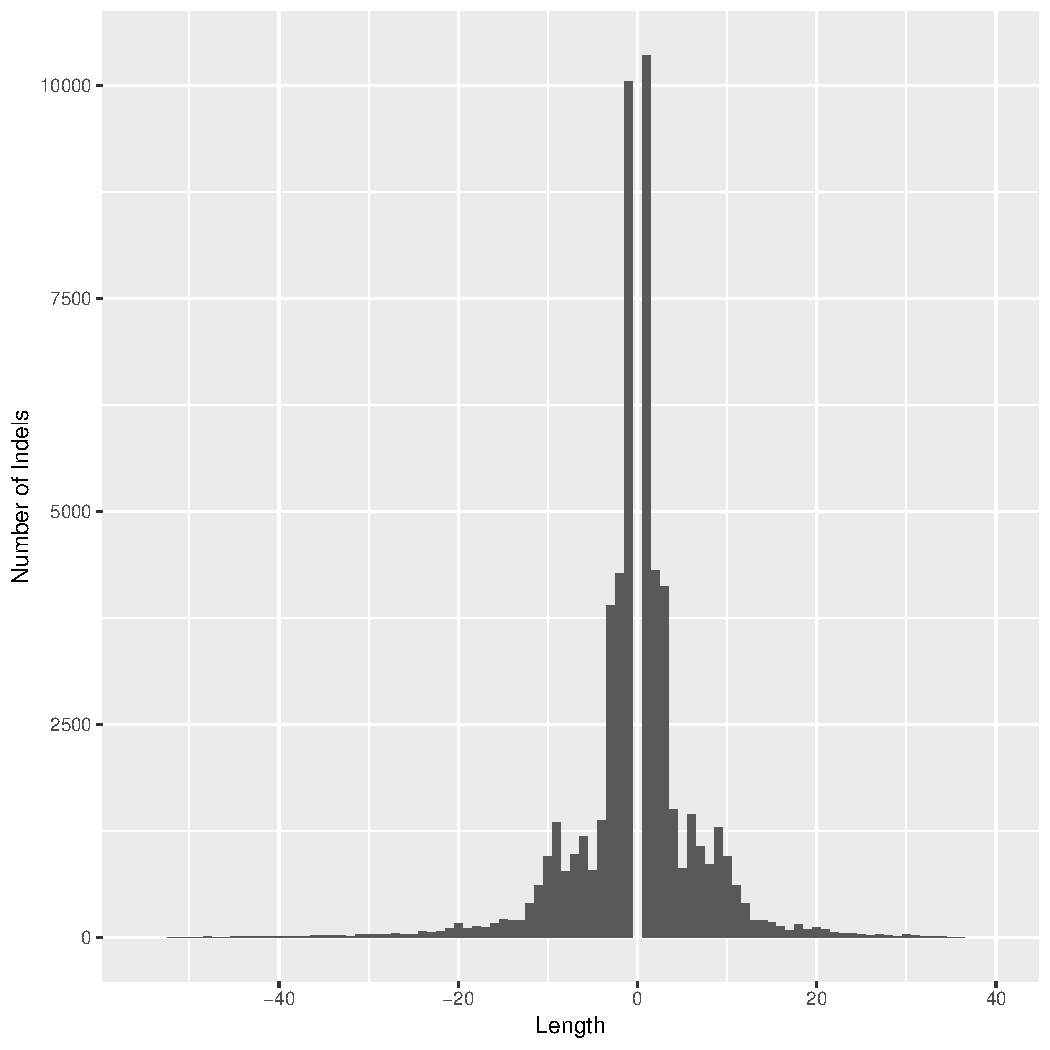
\includegraphics[angle=0,width=0.75\linewidth]{Figures/Ar109_histogram.pdf}}
		\resizebox{78mm}{78mm}{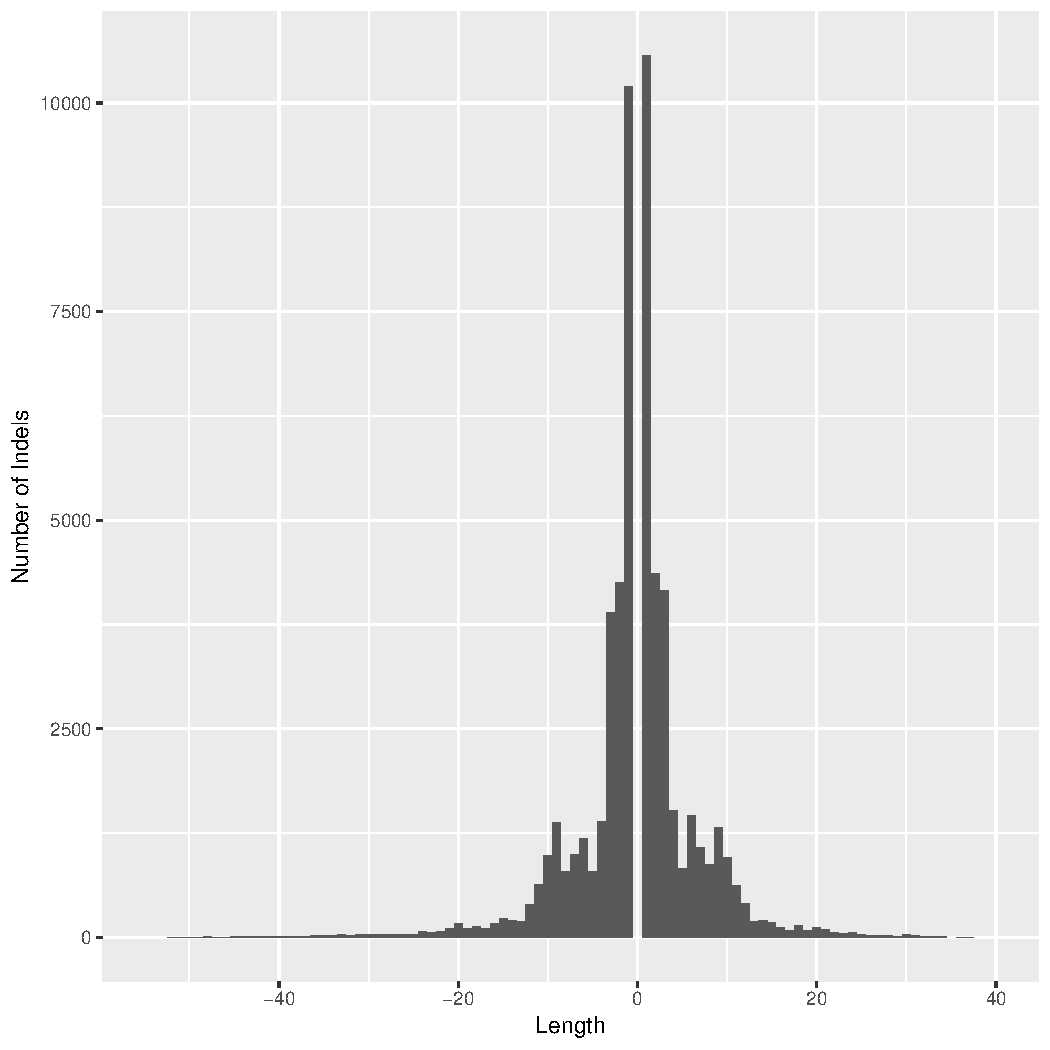
\includegraphics[angle=0,width=0.75\linewidth]{Figures/Ar119_histogram.pdf}}\\
		\resizebox{78mm}{78mm}{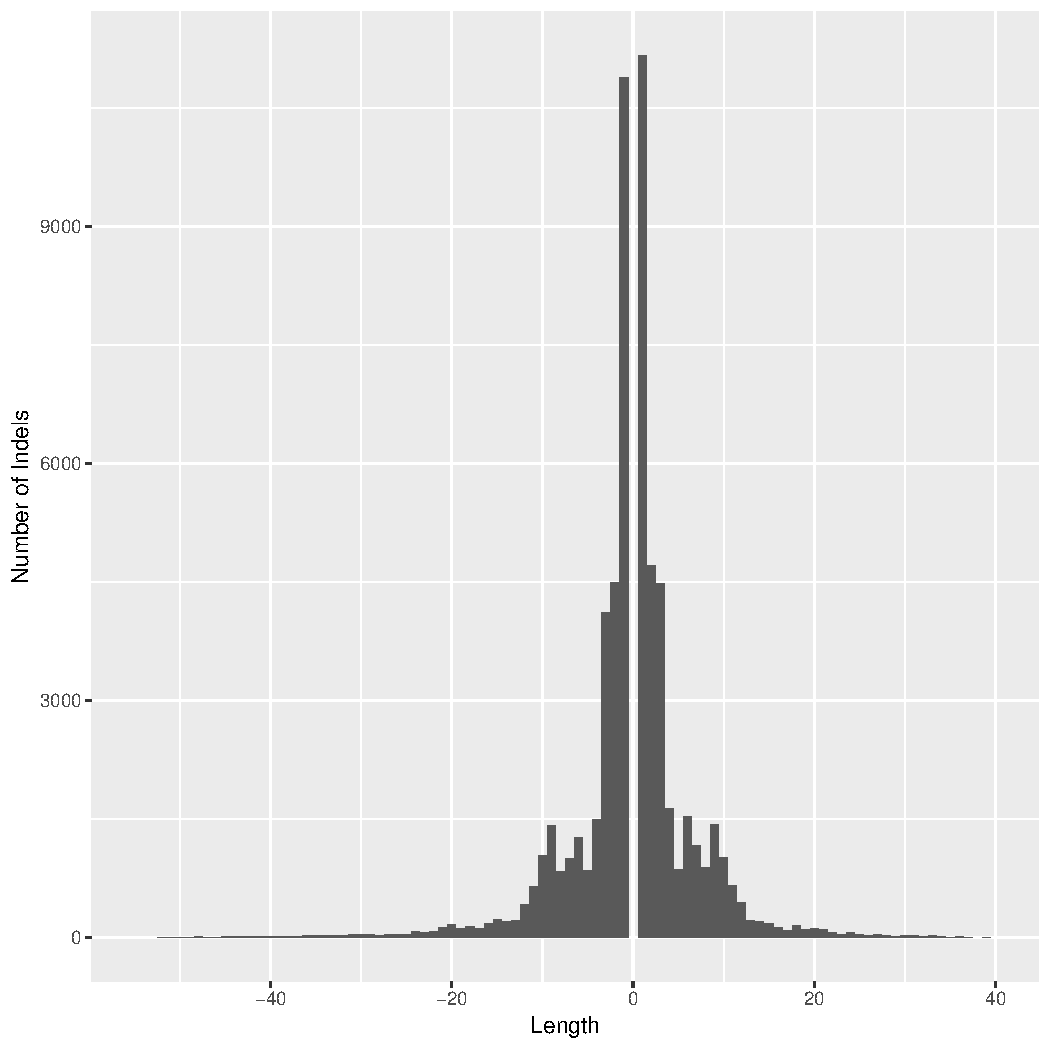
\includegraphics[angle=0,width=1.0\linewidth]{Figures/Ar142_histogram.pdf}}
		\resizebox{78mm}{78mm}{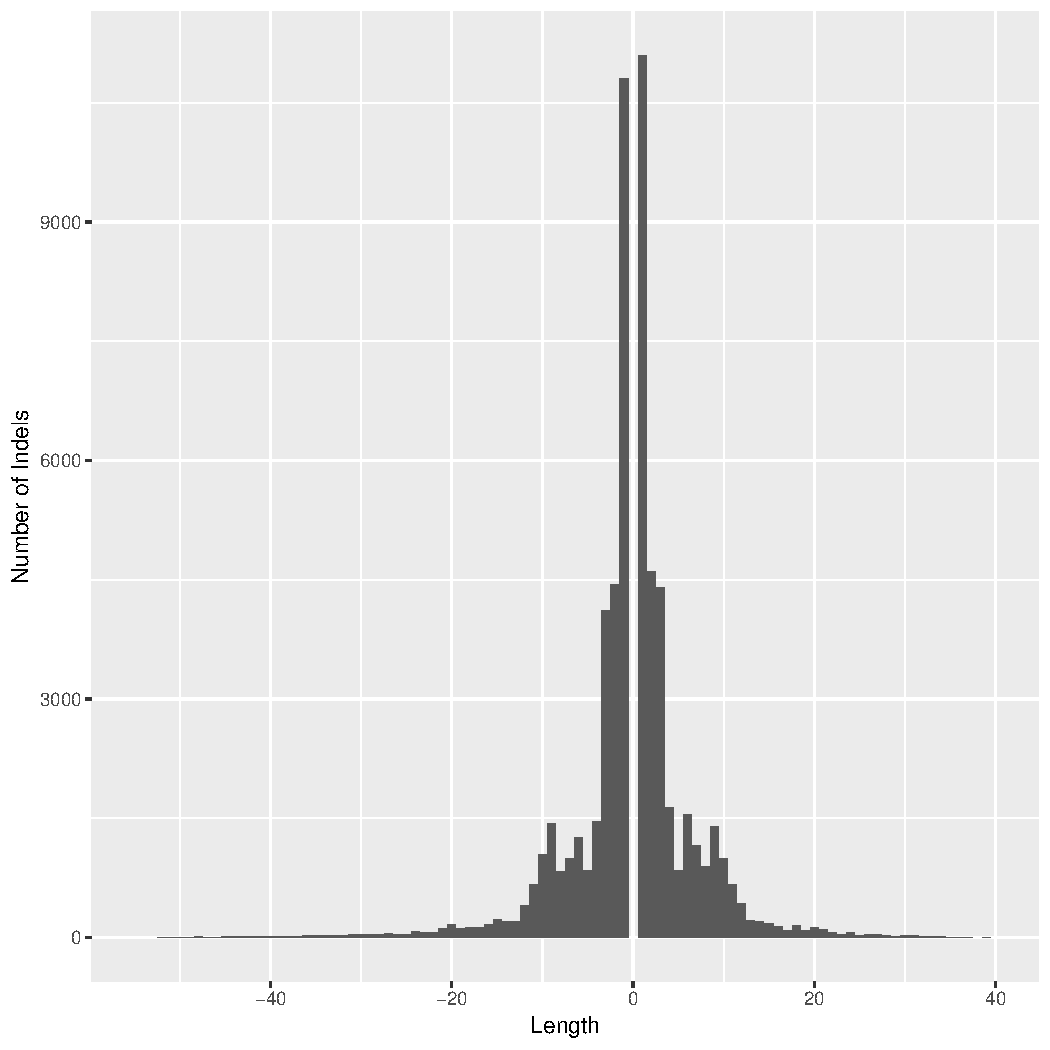
\includegraphics[angle=0,width=1.0\linewidth]{Figures/Ar159_histogram.pdf}}\\
		\resizebox{78mm}{78mm}{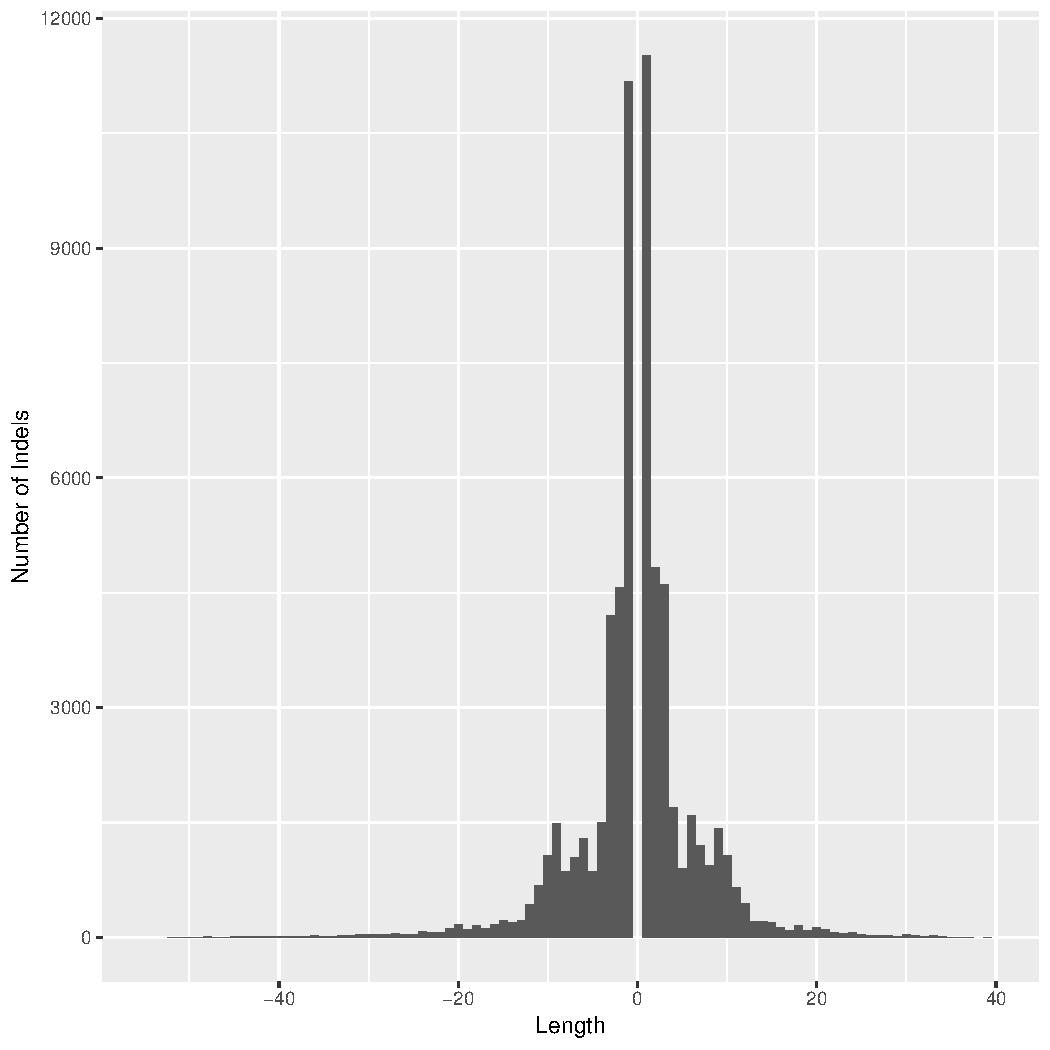
\includegraphics[angle=0,width=1.0\linewidth]{Figures/Ar170_histogram.pdf}}
		\resizebox{78mm}{78mm}{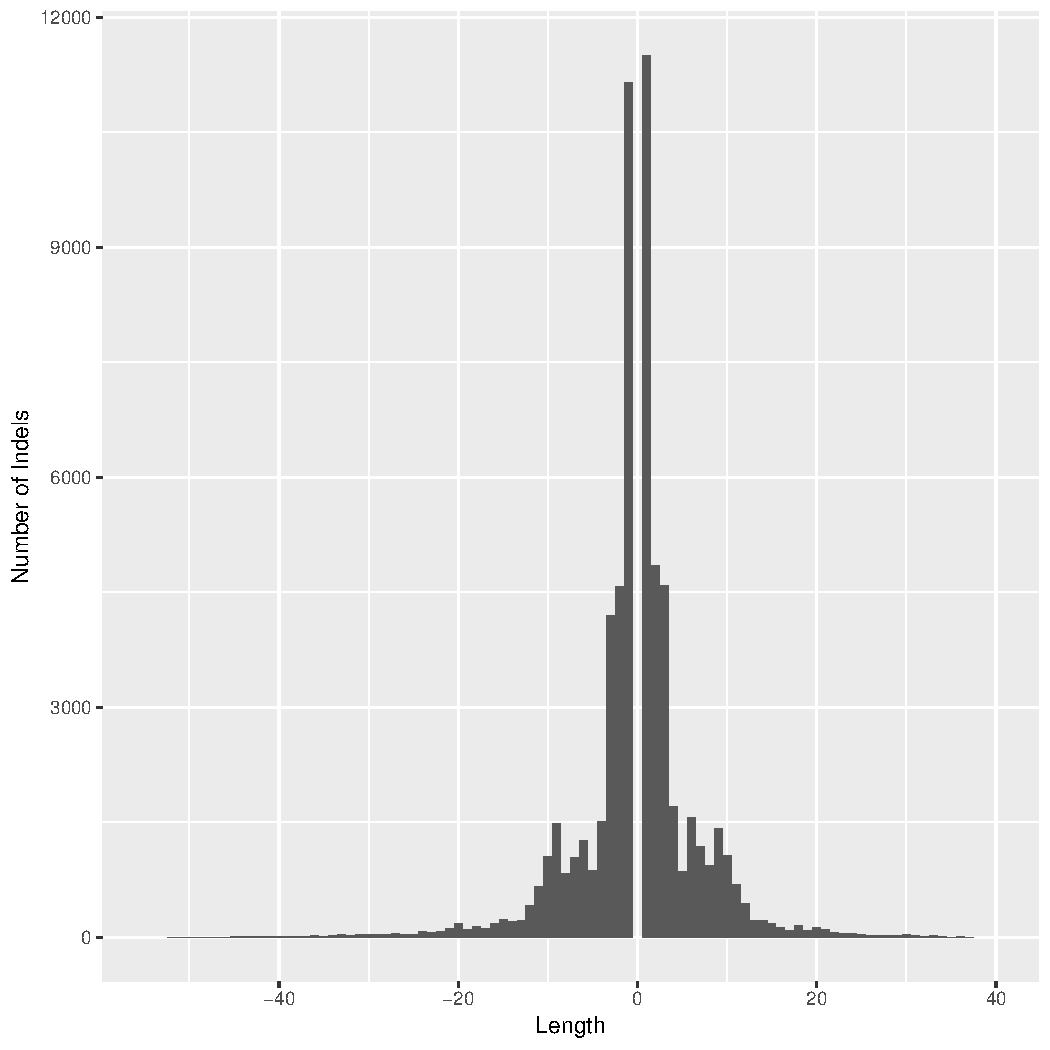
\includegraphics[angle=0,width=1.0\linewidth]{Figures/Ar174_histogram.pdf}}\\
		\begin{singlespace}
			\vspace{-0.5cm}
			\caption[The Frequency of the Indel Length]{The Frequency of the Indel Length Per Strain, Ar: 109, 119, 142, 159, 170, and 174}\label{Length_Indel_His}
		\end{singlespace}
	\end{centering}
\end{figure}

\begin{figure}[H]
	\begin{centering}
		\vspace{-1.5cm}
		\resizebox{78mm}{78mm}{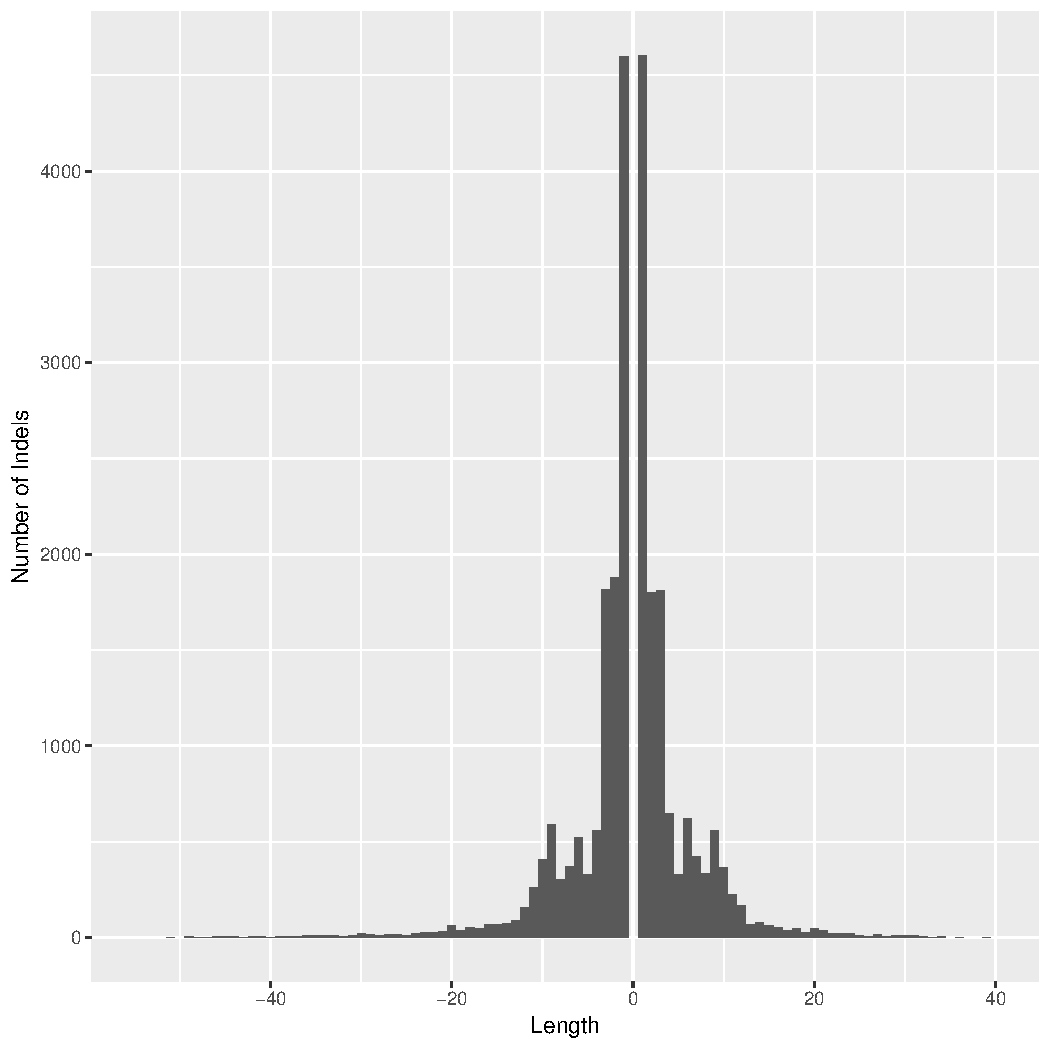
\includegraphics[angle=0,width=1.0\linewidth]{Figures/Ar175_histogram.pdf}}
		\resizebox{78mm}{78mm}{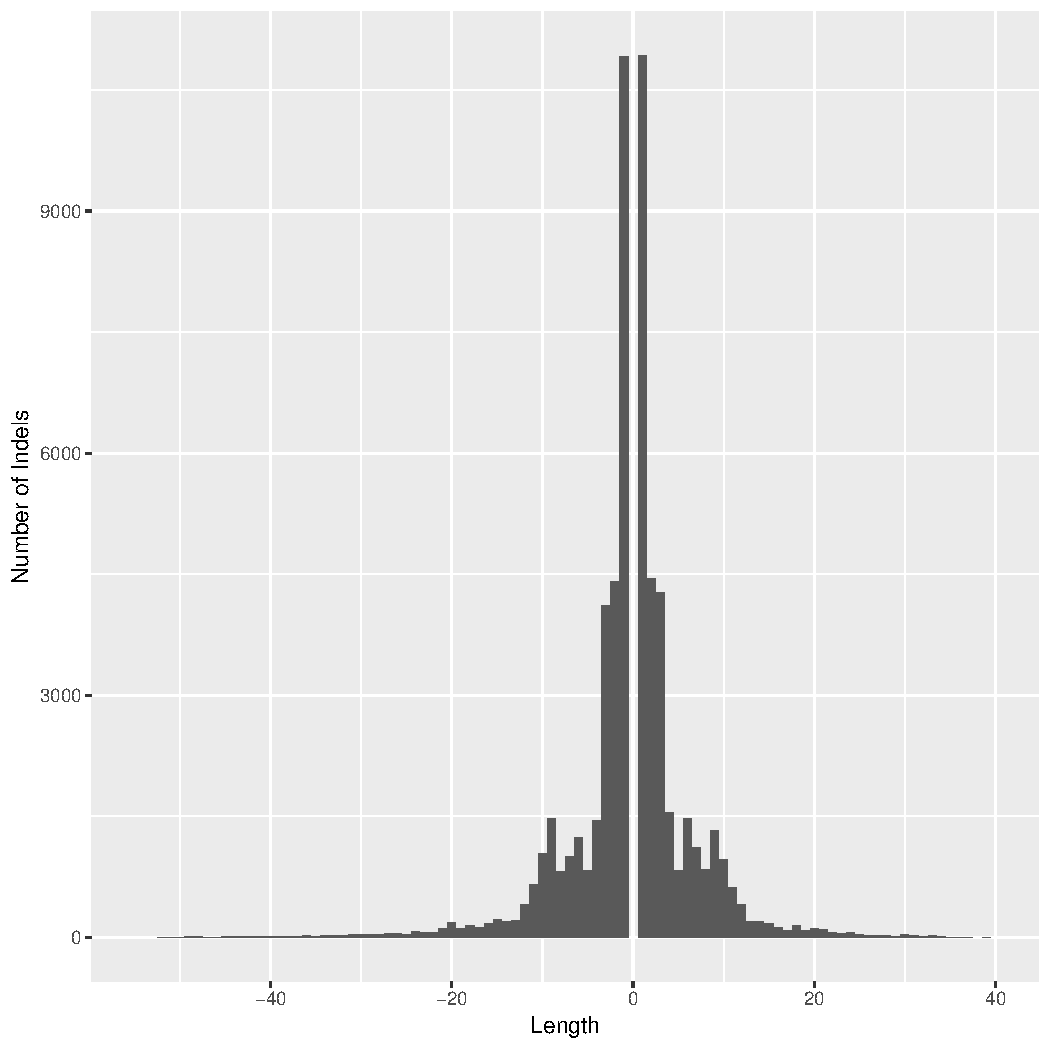
\includegraphics[angle=0,width=1.0\linewidth]{Figures/Ar176_histogram.pdf}}\\
		 \resizebox{78mm}{78mm}{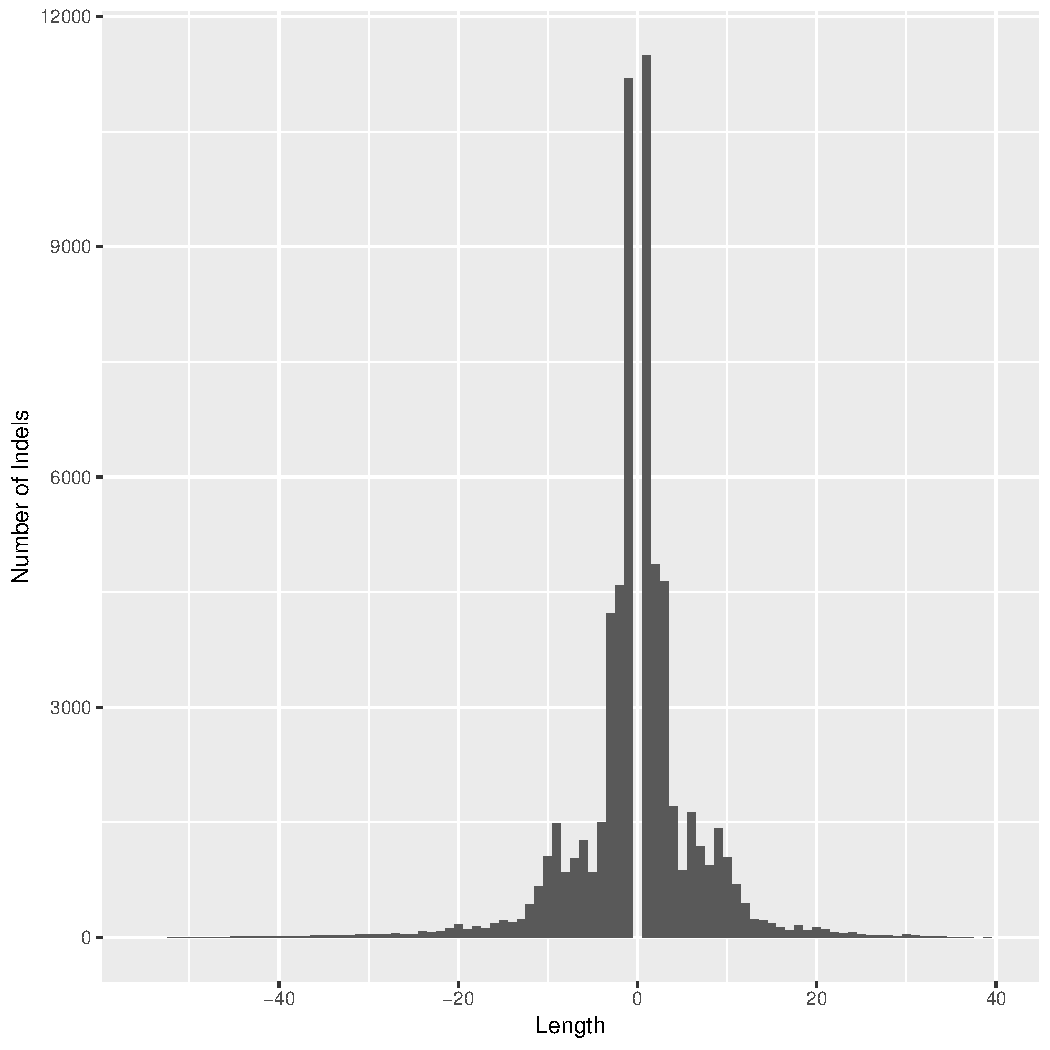
\includegraphics[angle=0,width=1.0\linewidth]{Figures/Ar179_histogram.pdf}}
		\resizebox{78mm}{78mm}{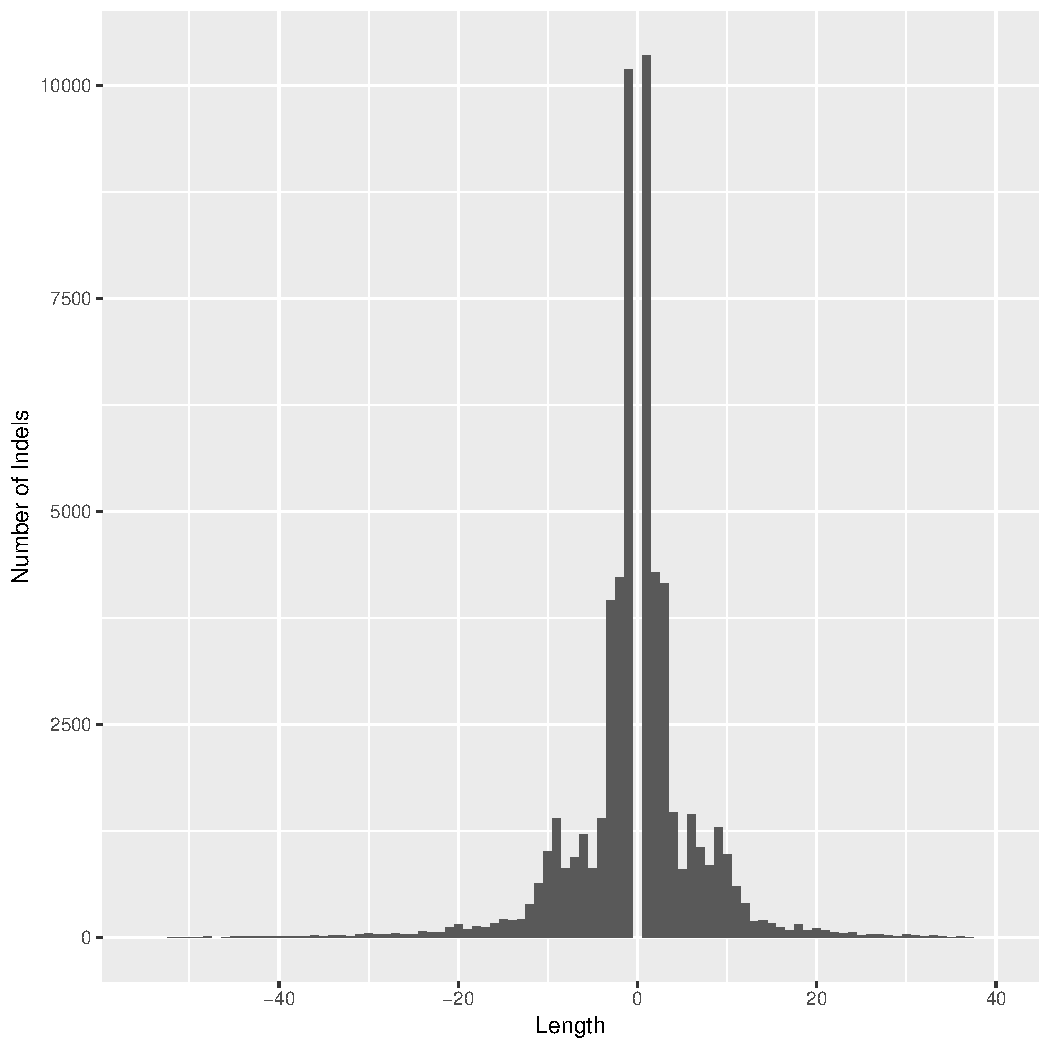
\includegraphics[angle=0,width=1.0\linewidth]{Figures/Ar188_histogram.pdf}}\\
		\resizebox{78mm}{78mm}{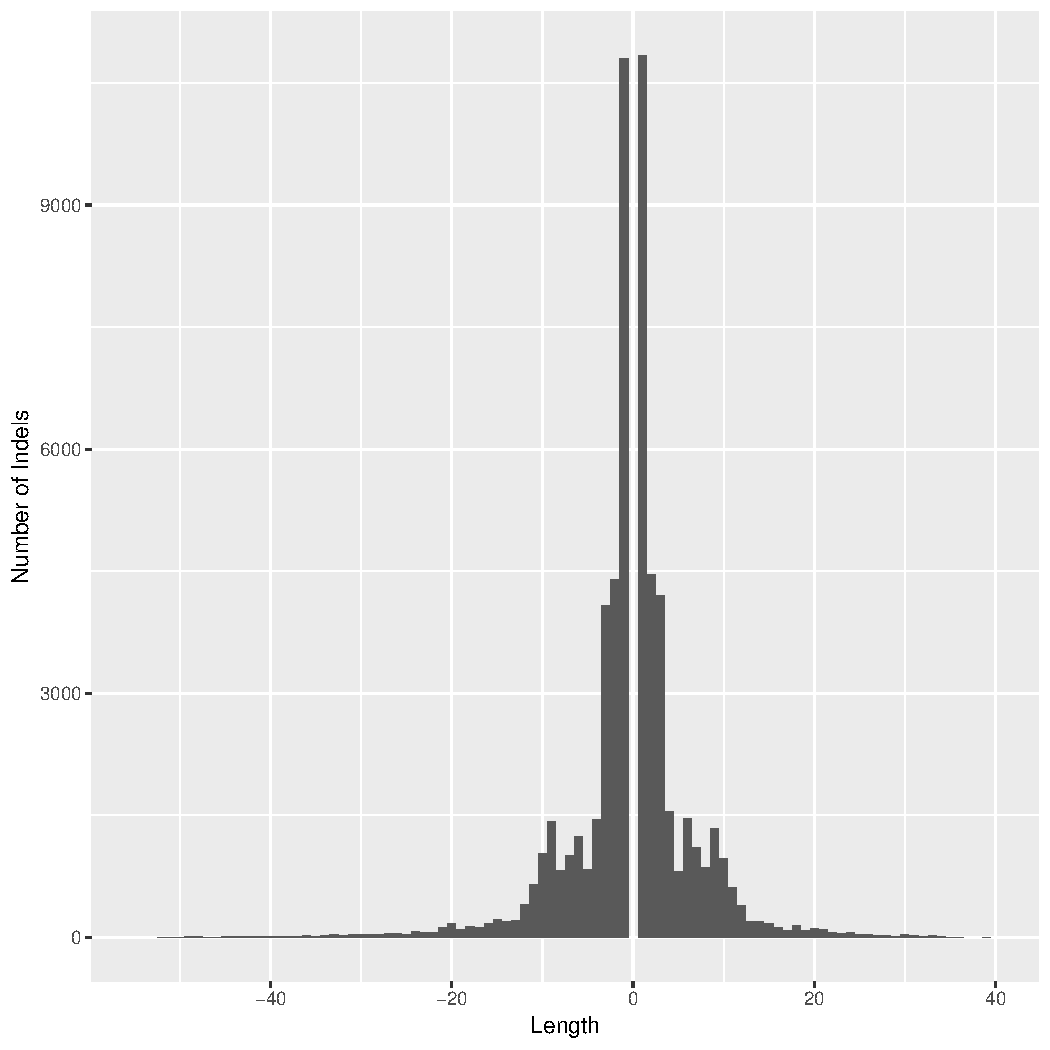
\includegraphics[angle=0,width=1.0\linewidth]{Figures/Ar194_histogram.pdf}}
		\resizebox{78mm}{78mm}{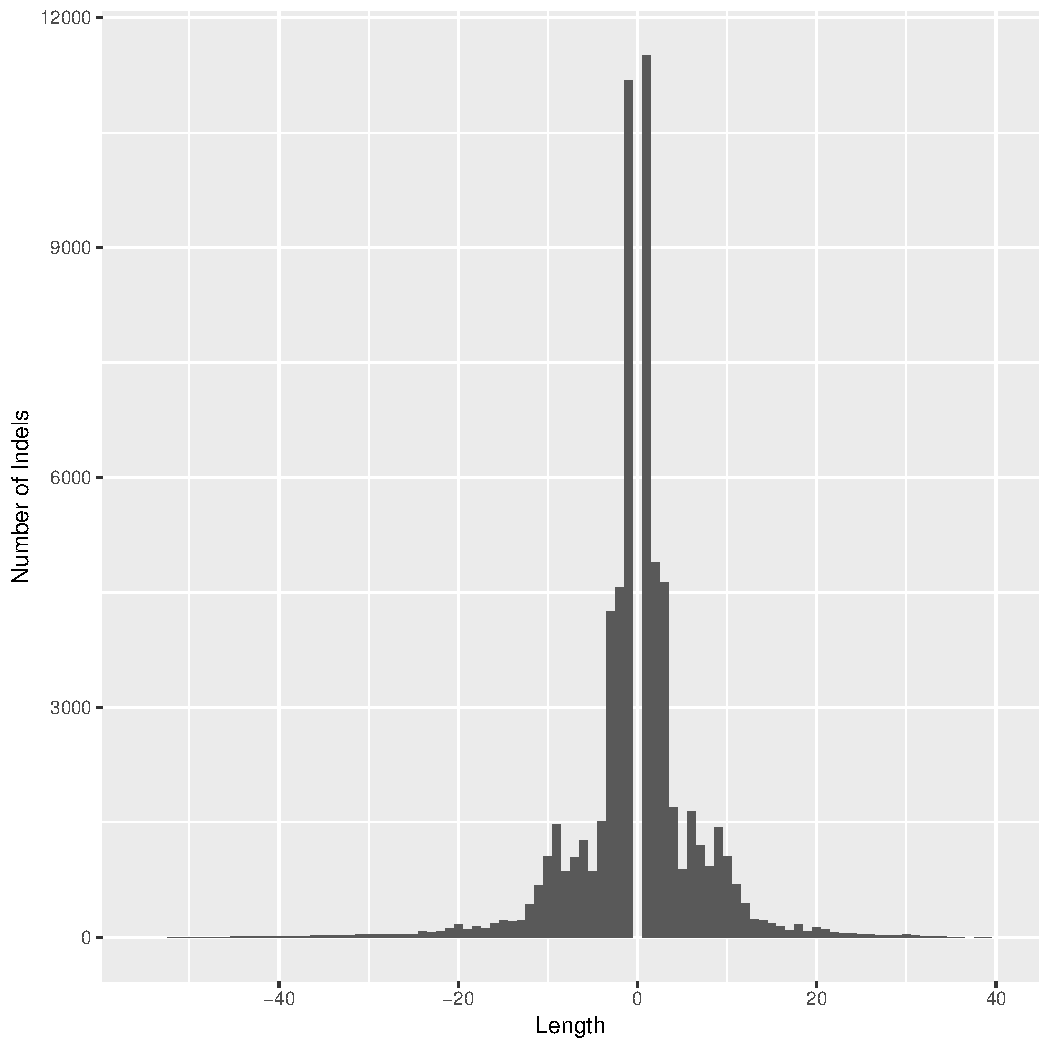
\includegraphics[angle=0,width=1.0\linewidth]{Figures/Ar196_histogram.pdf}}\\
		\begin{singlespace}
			\vspace{-0.5cm}
			\caption[The Frequency of the Indel Length2]{The Frequency of the Indel Length Per Strain, Ar: 175, 176, 179, 188, 194, and 196}\label{Length_Indel_His2}
		\end{singlespace}
	\end{centering}
\end{figure}

\begin{figure}[H]
	\begin{centering}
		\vspace{1.5cm}
                \resizebox{78mm}{78mm}{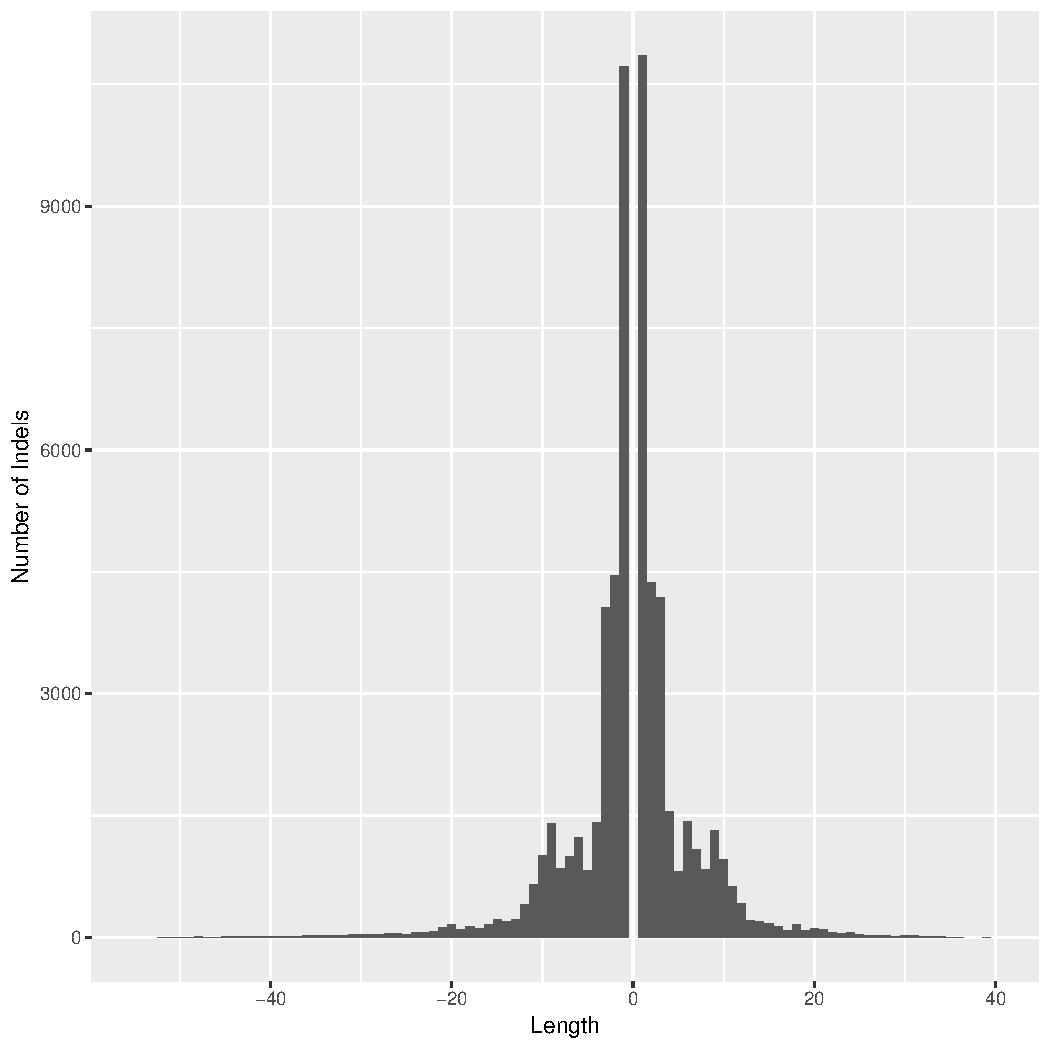
\includegraphics[angle=0,width=1.0\linewidth]{Figures/Ar201_histogram.pdf}}
		\resizebox{78mm}{78mm}{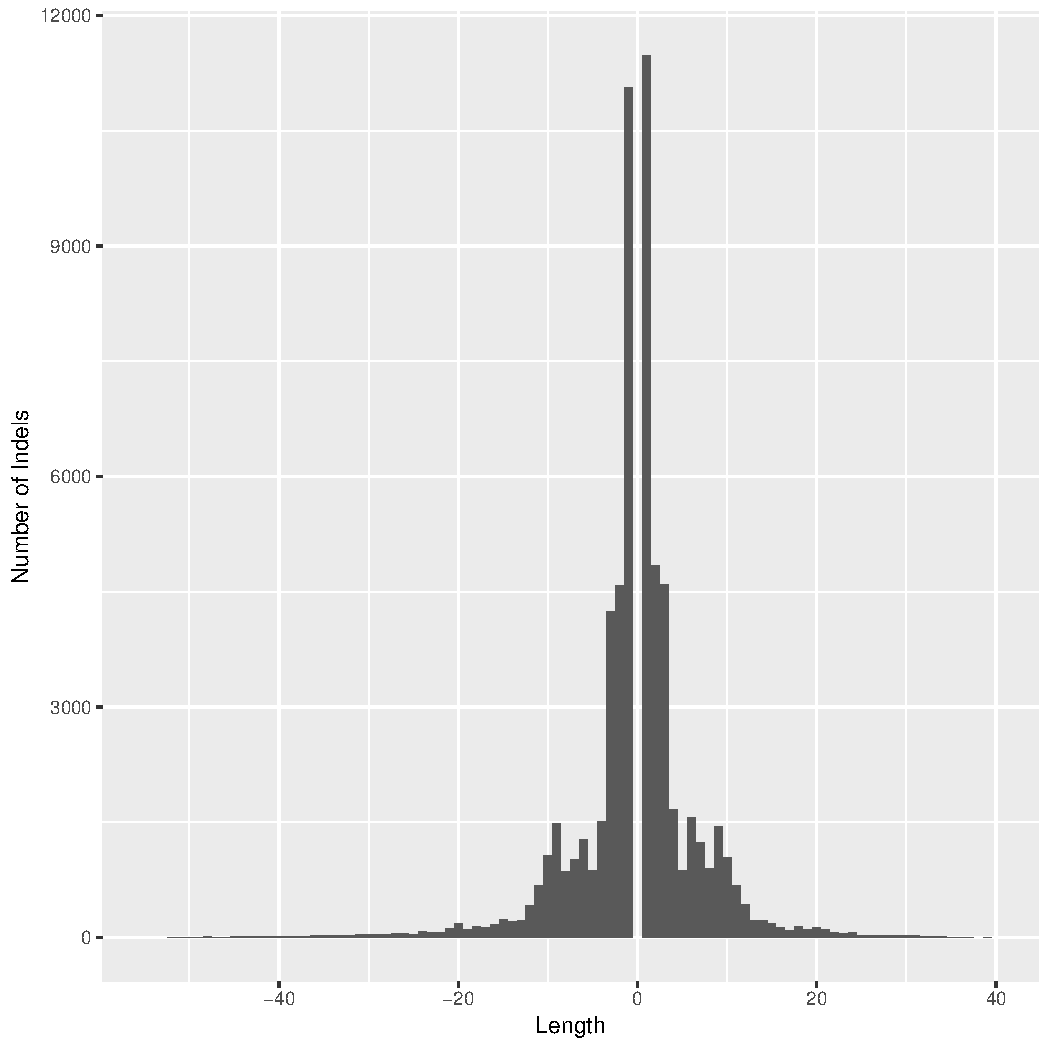
\includegraphics[angle=0,width=1.0\linewidth]{Figures/Ar213_histogram.pdf}}\\
		\resizebox{78mm}{78mm}{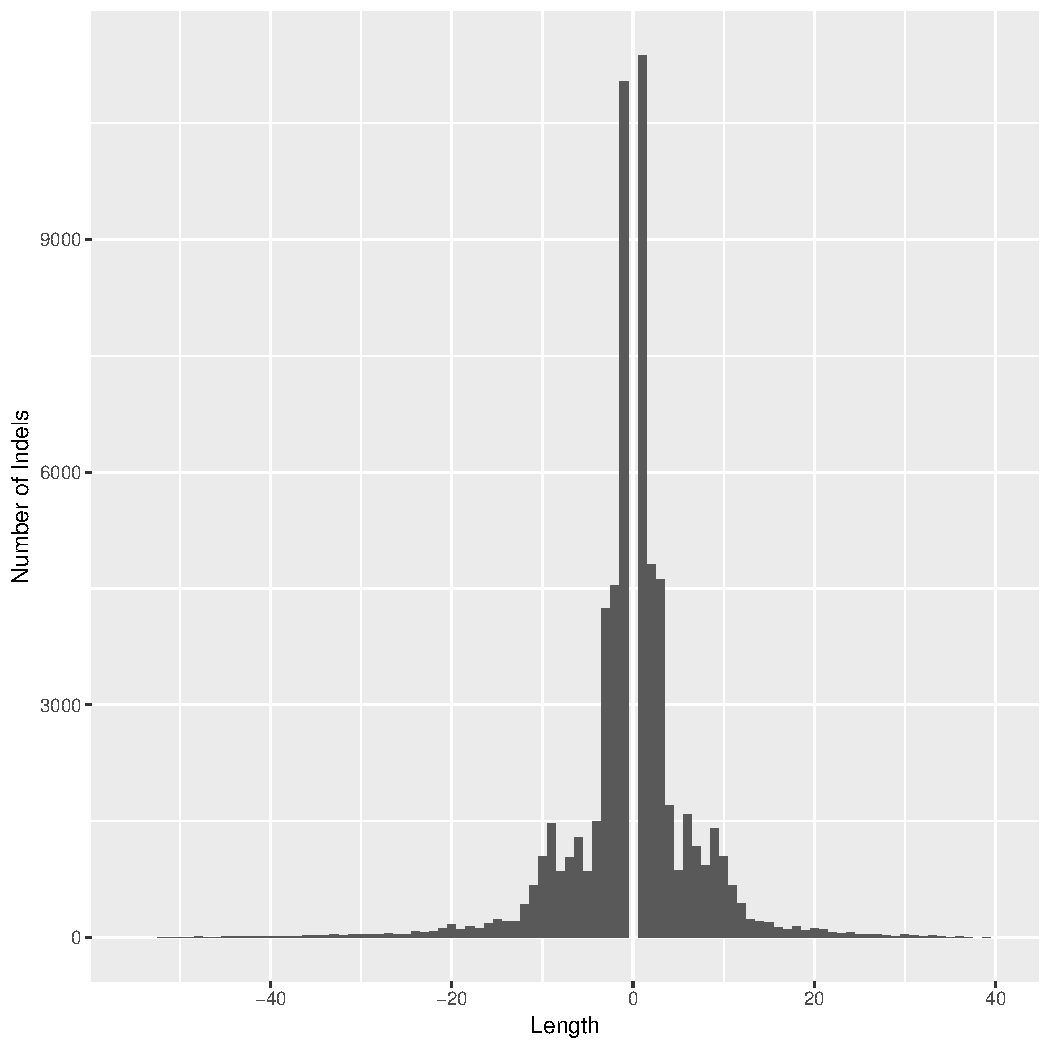
\includegraphics[angle=0,width=1.0\linewidth]{Figures/Ar73_histogram.pdf}}
		\begin{singlespace}
			 \vspace{-0.5cm}	
	\caption[The Frequency of the Indel Length3]{The Frequency of the Indel Length Per Strain, Ar: 201, 213, and73}\label{Length_Indel_His3}
		\end{singlespace}
	\end{centering}
\end{figure}
	
\begin{figure}[H]
	\begin{centering}
		\vspace{1.5cm}
		\resizebox{78mm}{78mm}{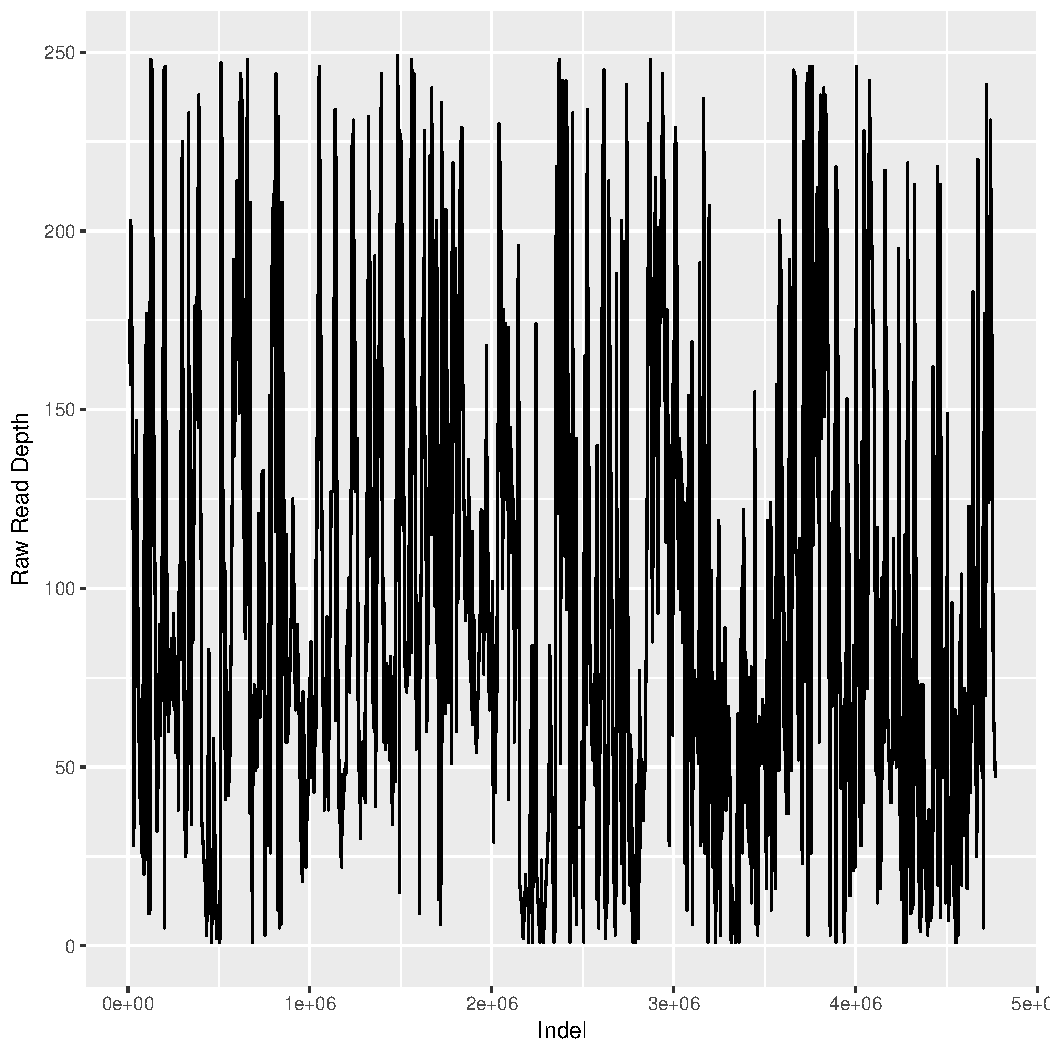
\includegraphics[angle=0,width=1.0\linewidth]{Figures/1_DP_locations.pdf}}
                \resizebox{78mm}{78mm}{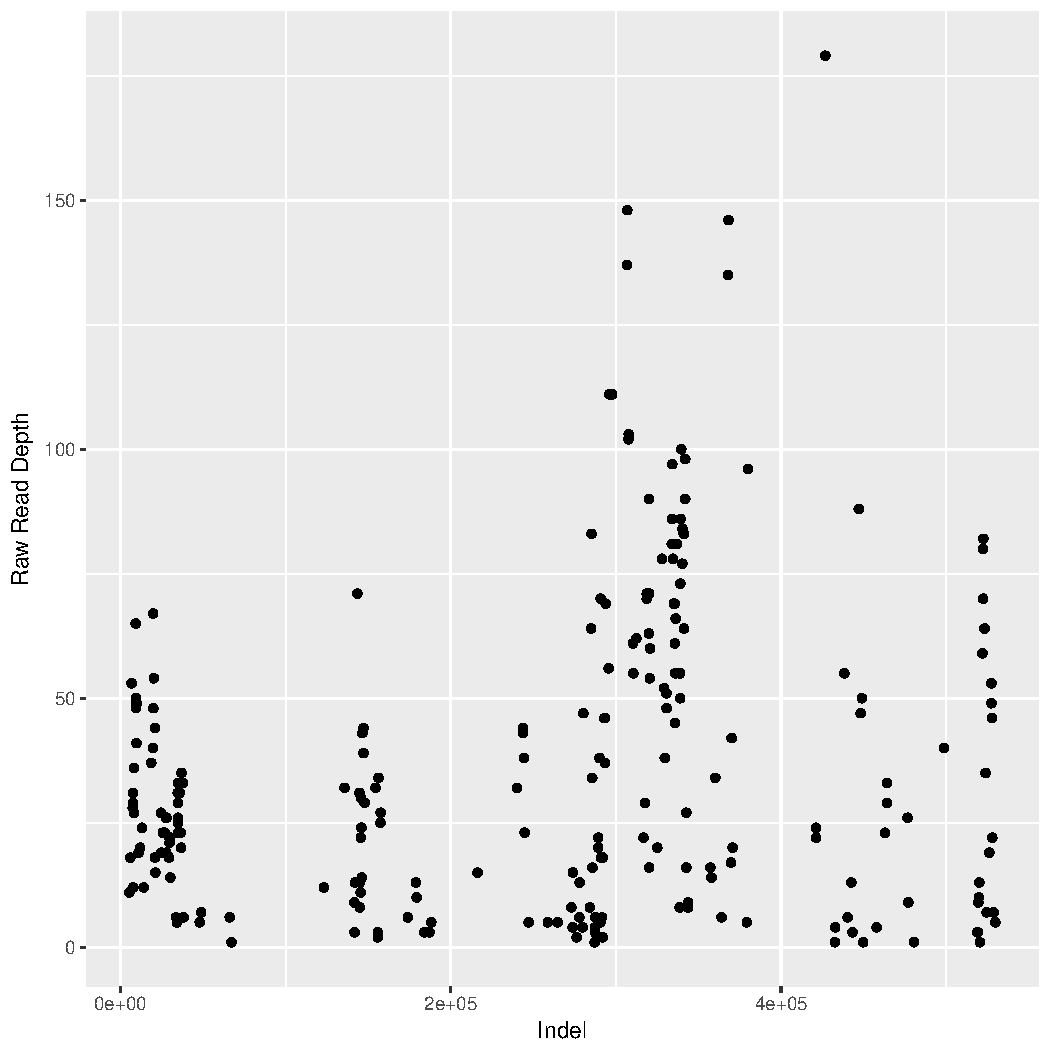
\includegraphics[angle=0,width=1.0\linewidth]{Figures/50_DP_locations.pdf}}\\
		\resizebox{78mm}{78mm}{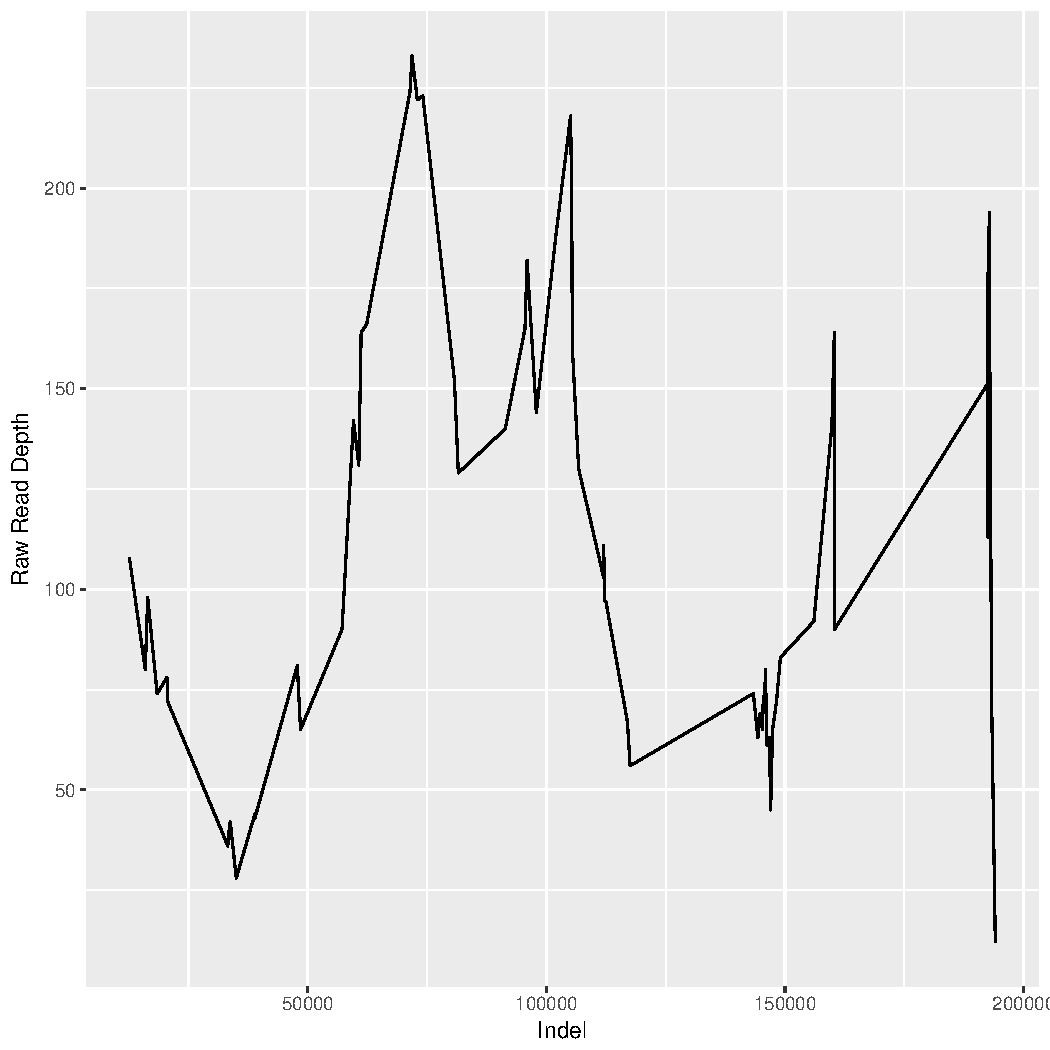
\includegraphics[angle=0,width=1.0\linewidth]{Figures/100_DP_locations.pdf}}
		\begin{singlespace}
		    \vspace{-0.5cm}	
		    \caption[The Read Depth of Indels Found]{The Read Depth of Indels Found in Ar:109 at Scaffold:1, 50, and 100}\label{readdepth_indel}
	   \end{singlespace}
	\end{centering}
\end{figure}







\end{document}
